\section*{}
\begin{center}
    {\fontsize{14}{1.5}\selectfont \textbf{CHAPTER VI}}\\
    \vspace{12pt}
    {\fontsize{16}{1.5}\selectfont \textbf{Findings and Recommendations}}\\
    \vspace{12pt}
    \vspace{12pt}
\end{center}

\setcounter{section}{6}
\setcounter{subsection}{0}
\addcontentsline{toc}{section}{\textbf{CHAPTER VI Findings and Recommendations }} % Add to ToC

\subsection{Findings}{




\subsubsection{Enhanced Accuracy with Long-term History Integration:
}
   The E2E-LOAD model demonstrates that incorporating long-term historical data significantly boosts the accuracy of online action detection. This improvement is achieved through the Long-term Compression LC and Long-Short term Fusion LSF modules which integrate long-term historical data into short-term memory for better spatiotemporal modeling. By combining both long-term and short-term data the model achieves impressive performance metrics including a mean average precision mAP of 72.4 percent.

\subsubsection{ Efficiency Gains through Efficient Inference Technique:
}
   The Efficient Inference EI technique introduced in the E2E-LOAD model significantly enhances processing speed without sacrificing accuracy. By accelerating the spatiotemporal attention process the model achieves a substantial increase in frames per second FPS enhancing its real-time detection capabilities. For example incorporating EI increased the FPS from 9.1 to 19.5 in the baseline configuration demonstrating the techniques effectiveness in optimizing performance.

\subsubsection{Superior Accuracy with IDN Model:
}
   The Information Discrimination Network IDN surpasses existing state-of-the-art methods in online action detection by effectively distinguishing relevant information from irrelevant data. This ability allows the IDN model to achieve higher mean class accuracy performance mcAP with IDN-Kinetics reaching up to 86.1 percent mcAP. The models design reduces false detections by enhancing the discrimination of action-relevant information significantly contributing to its superior performance.

\subsubsection{Early Action Detection Capability:
}
   In online action detection identifying actions as early as possible is crucial. The IDN model excels in this aspect consistently maintaining high accuracy throughout action progression and showing significant improvements in early action detection segments compared to other models. This early detection capability is vital for real-time applications where prompt response to actions is necessary.

 
\subsection{Recommendations}

\subsubsection{ Integrate Long-term and Short-term Data:
}
 To enhance the performance of online action detection systems it is recommended to integrate long-term historical data with short-term memory. As demonstrated by the E2E-LOAD model this approach can significantly improve the accuracy of detecting ongoing actions. Implementing modules such as Long-term Compression LC and Long-Short-term Fusion LSF can provide a more comprehensive spatiotemporal context leading to better detection results.

\subsubsection{ Adopt Efficient Inference Techniques for Real-time Applications:
}
   Incorporating Efficient Inference EI techniques is crucial for applications requiring real-time action detection. By optimizing the spatiotemporal attention process these techniques can enhance processing speed and ensure timely detection without sacrificing accuracy. This is particularly important for systems deployed in dynamic environments where immediate action recognition is necessary.

\subsubsection{ Focus on Information Discrimination:
}
   Developing models that can effectively discriminate between relevant and irrelevant information is essential for improving detection accuracy. The success of the IDN model highlights the importance of enhancing information discrimination capabilities. Future models should incorporate mechanisms to filter out irrelevant data thereby reducing false positives and improving overall detection performance.

\subsubsection{Prioritize Early Detection Capabilities:
}
   Ensuring that models can accurately detect actions at the earliest stages is vital for many real-time applications. Enhancing early detection capabilities can lead to more responsive and proactive systems. It is recommended to design and train models with a focus on early action recognition possibly through specialized loss functions or training regimes that emphasize the importance of initial action segments.

By implementing these recommendations the development and deployment of online action detection systems can achieve higher accuracy efficiency and responsiveness effectively meeting the demands of real-world applications.

}


\vspace{12pt}
\vspace{12pt}
\vspace{12pt}

\begin{figure}[htbp]
    \centering
    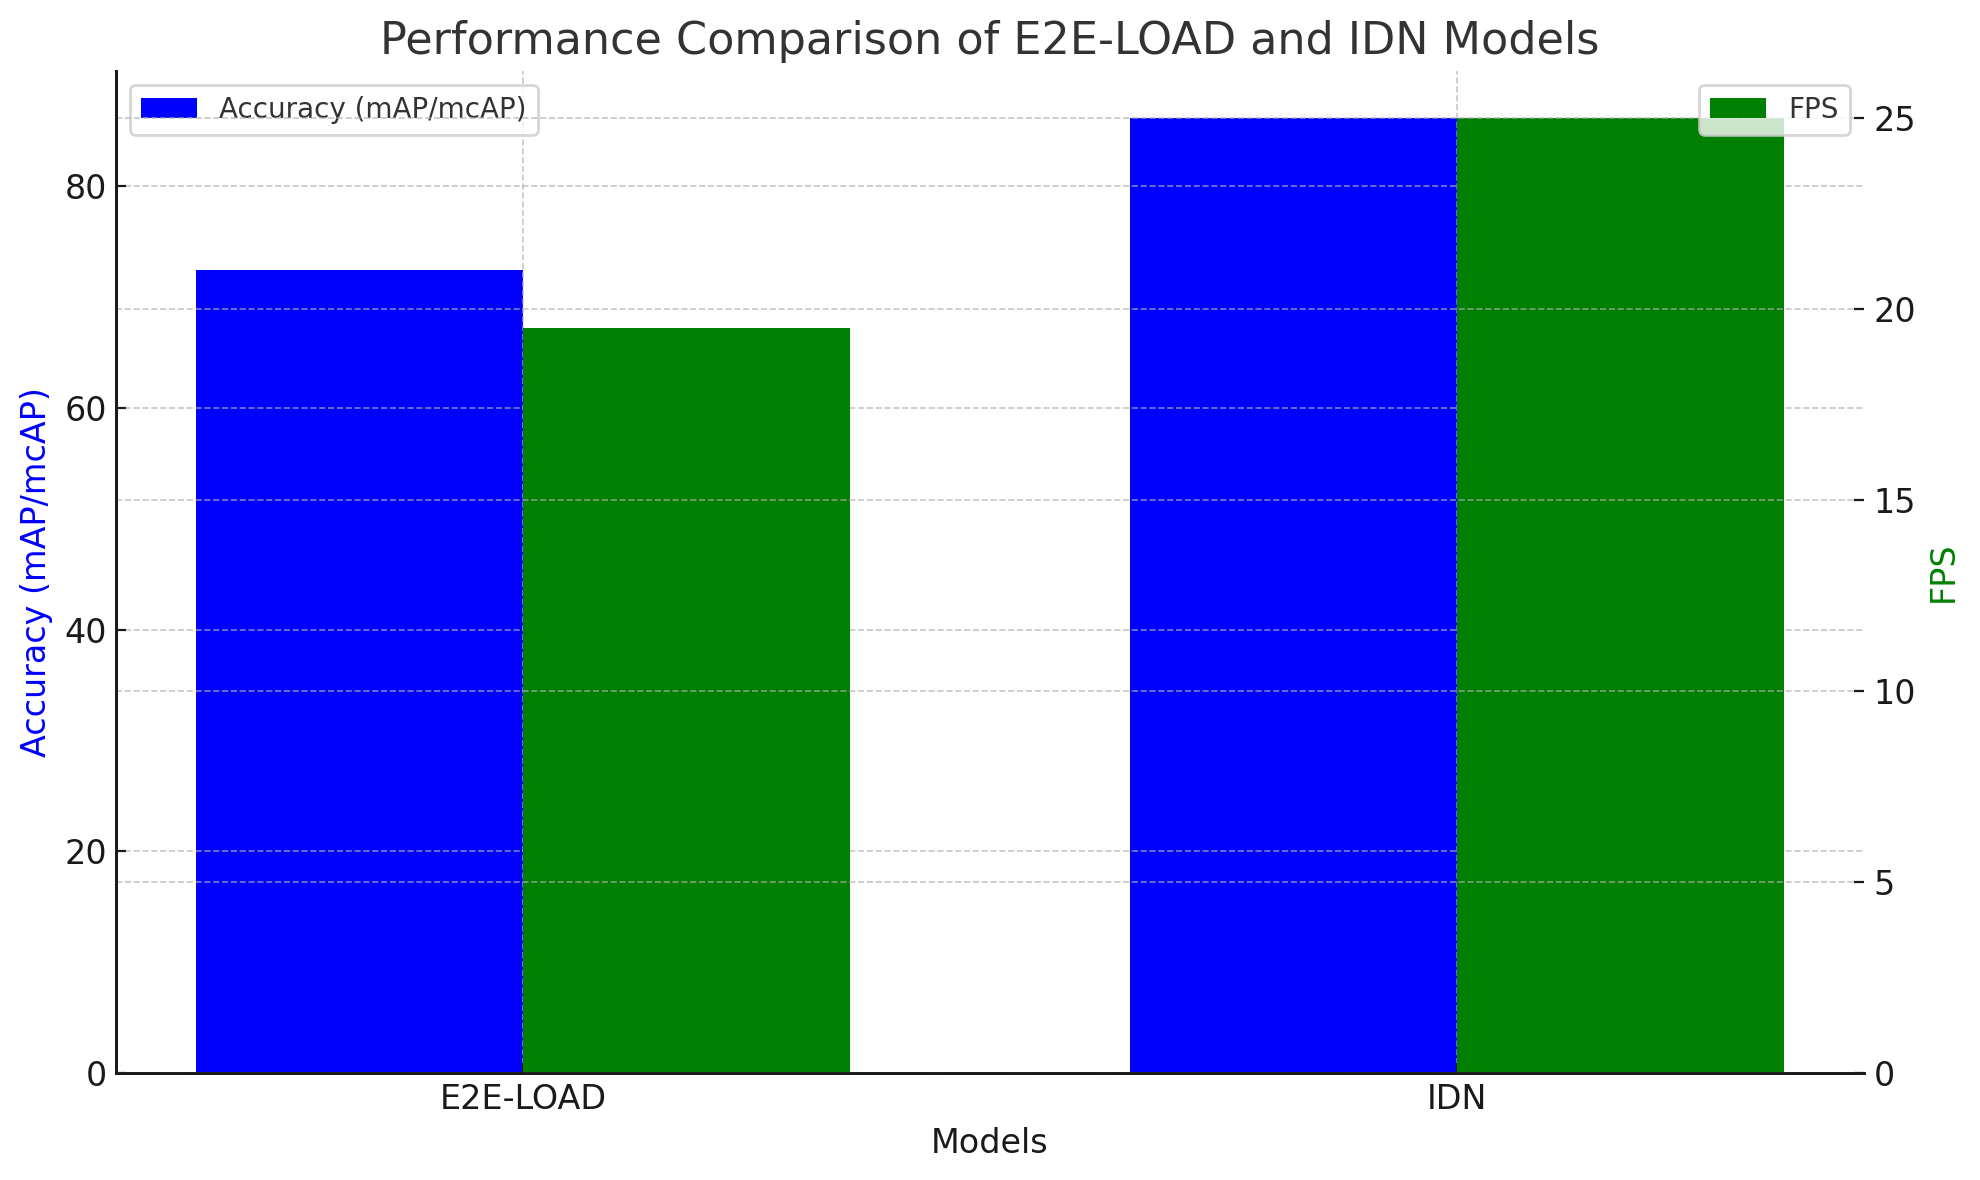
\includegraphics[width=6in]{img/performance.png}
    \caption{Performance Comparison}
    \label{fig:example}
\end{figure}
